\documentclass[10pt]{article}

\usepackage{float}

\usepackage{fancyhdr} % Required for custom headers

\usepackage{lastpage} % Required to determine the last page for the footer

\usepackage{extramarks} % Required for headers and footers

\usepackage{graphicx} % Required to insert images

\usepackage{lipsum} % Used for inserting dummy 'Lorem ipsum' text into the template

\usepackage{setspace} % Line spacing

\usepackage[title]{appendix}

\usepackage{indentfirst}

\usepackage{helvet}

\usepackage{varioref}

\usepackage{hyperref}

\usepackage{cleveref}

\renewcommand{\familydefault}{\sfdefault}



% Margins

\setlength\parindent{24pt}

\topmargin=-0.45in

\evensidemargin=-.25in

\oddsidemargin=-.25in

\textwidth=7.0in

\textheight=9.0in

\headsep=0.25in 



\onehalfspacing

\newcommand{\quotes}[1]{``#1''}



% Set up the header and footer

\pagestyle{fancy}

\lhead{\firstxmark} % Top right header

\chead{\projecttitle} % Top left header

\rhead{\lastxmark} % Top right header

\lfoot{\firstxmark} % Bottom left footer

\rfoot{Page\ \thepage\ of\ \pageref{LastPage}} % Bottom right footer

\renewcommand\headrulewidth{0.4pt} % Size of the header rule

\renewcommand\footrulewidth{0.4pt} % Size of the footer rule



\setlength\parindent{0pt} % Removes all indentation from paragraphs

   

%----------------------------------------------------------------------------------------

%	NAME AND CLASS SECTION

%----------------------------------------------------------------------------------------



\newcommand{\projecttitle}{MDDS OS \\ User Guide} % Project Title

\newcommand{\hmwkAuthorName}{Yuchen Tian and Michael Tran} % Your name



%----------------------------------------------------------------------------------------

%	TITLE PAGE

%----------------------------------------------------------------------------------------



\title{
\vspace{2in}
\textmd{\textbf{\projecttitle} \\}
\vspace{5in}
}



\author{\textbf{\hmwkAuthorName}}

\date{} % Insert date here if you want it to appear below your name



%----------------------------------------------------------------------------------------



\begin{document}



\maketitle



%----------------------------------------------------------------------------------------

%	TABLE OF CONTENTS

%----------------------------------------------------------------------------------------



\newpage

\tableofcontents

\newpage



%----------------------------------------------------------------------------------------

%	Intro

%----------------------------------------------------------------------------------------



%----------------------------------------------------------------------------------------

%	Intro

%----------------------------------------------------------------------------------------



\section{Introduction}

\begin{figure}[H]
	\centering
	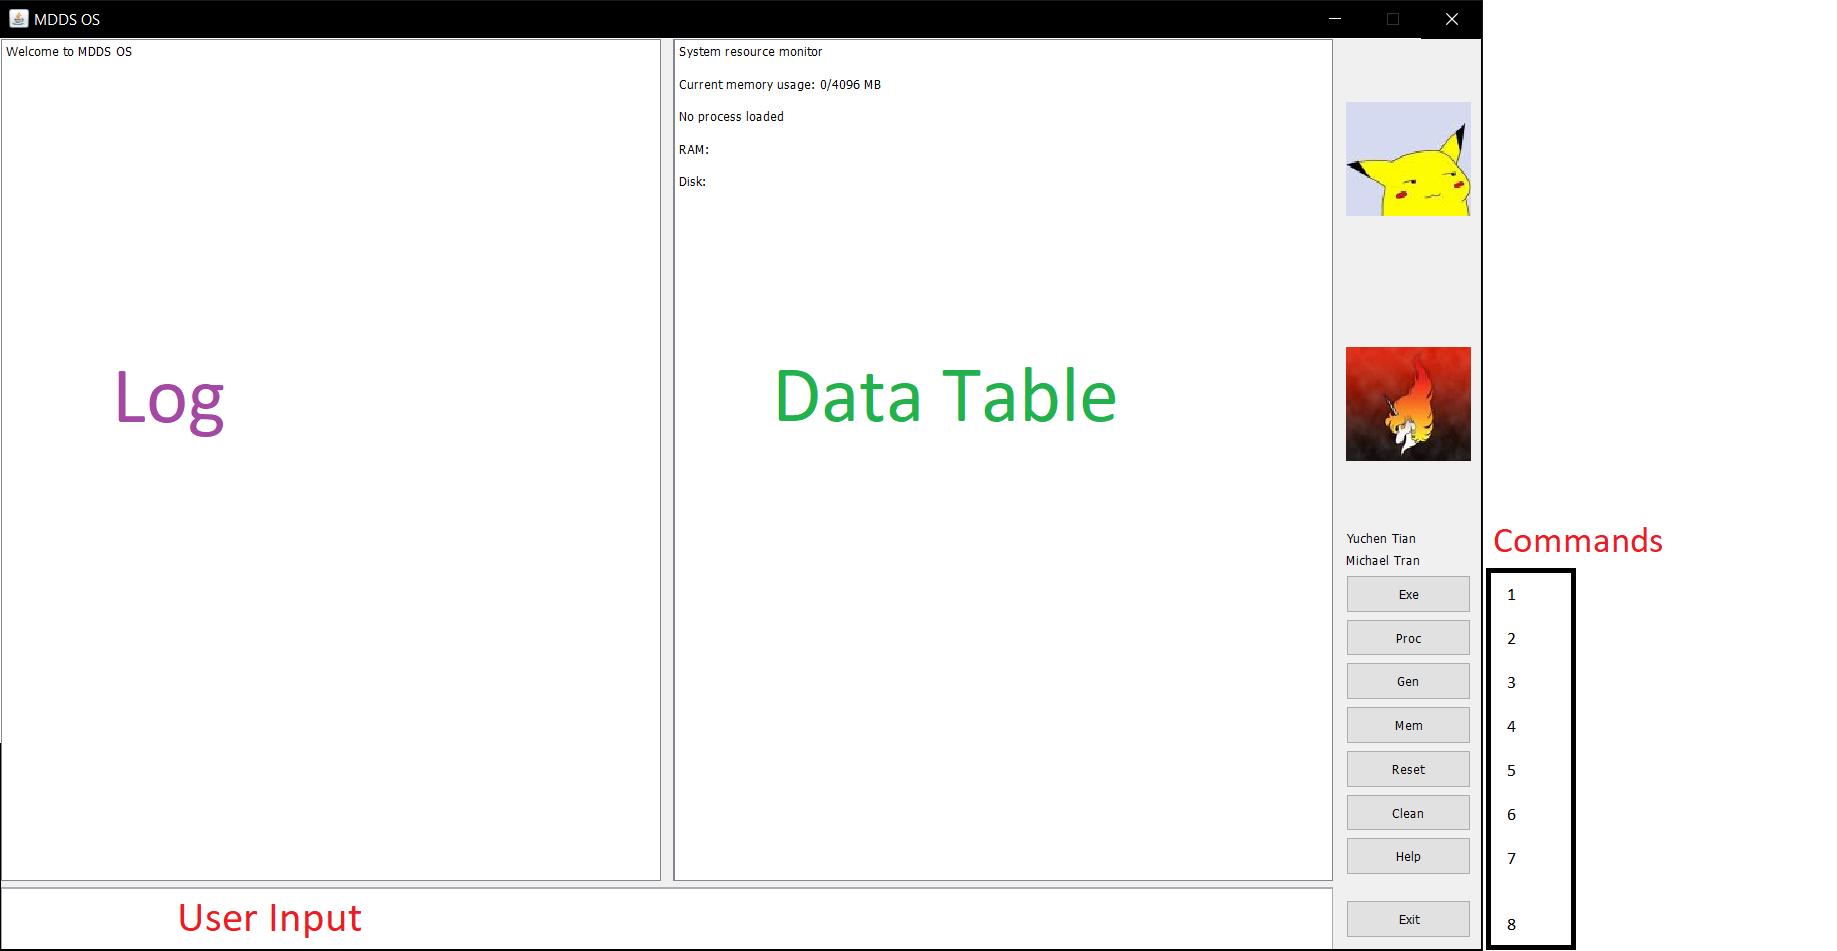
\includegraphics[width=\linewidth]{Untitled}
\end{figure}


\section{Commands}

\subsection{Exe}




\end{document}
